\chapter{Evaluations and Results}
\markright{Aravindan Mahendiran \hfill Chapter 3. Evaluations and Results \hfill}
To evaluvate our hypothesis we test our models on different elections from Latin America.
The tweets are provided by DataSift, an infoveilence service that resells Twitter data.
On an average we collect close to 2 million unique tweets a day from over 21 countries in Latin and South America.
Then these tweets are geo-coded using a geo-location algorithm we developed to obtain tweets from the country of interest.
We then run the two prediction algorithms to get their baseline perfermance.
These two models have been tested extensively on 36 elections from Latin America from 2012-2013 including Presidential, Governor and Mayoral elections. 
Out of these 36 elections, the models predicted 21 of them correctly. 
%The combined track record for the two elections have been detailed in \ref{table:trackRecord}. 
Importantly every single election was predicted ahead of time and not in reterospect.
The models perform poorly on local mayoral elections(12 out of 24 predicted correctly) as there was not much chatter on Twitter about these elections to make sound predictions. 
The regression model was used only for presidential elections as opinion polls were not available for Governor and Mayoral elections.
Hence we use only the presidential elections to evaluavate our vocabulary.
Once we have the baseline score for these models, we then use the same vocabulary to seed our PSL learning algorithm. 
The prediction algorithms are then run again, now by using the expanded vocabulary obtained through the query expansion at each iteration.
%track record table

\begin{table*}[Ht]
	\centering
	\begin{tabular}{| r || r | r | r | r | r | r |}
 	\hline
 	Election & UniVis+Seed & UniVis+PSL & Improv. & Reg+Seed & Reg.+PSL & Improv\\
 	\hline
	Mexico & 0.353 & 0.368 & -4.2\% & 0.123 & 0.07 & 43.09\% \\ 	
 	Venezuela\_Oct7 & 0.069	& 0.077 & -11.59\% & 0.158 & 0.109 & 31.01\&\\
	Ecuador & 0.531 & 0.547 & -3.01\% & 0.263 & 0.244 & 7.22\% \\
	Venezuela\_Apr15 & 0.198 & 0.178 & 10.10\% & 0.142 & 0.112 & 21.126\&\\
	Paraguay & 0.34 & 0.288 & 15.29\% & 0.2 & 0.18 & 10\% \\
	Chile\_Nov17 & 0.56 & 0.42 & 25\% & 0.245 & 0.207 & 15.51\% \\
	Honduras & 0.563 & 0.527 & 6.39\% & 0.293 & 0.184 & 37.20\% \\
	Chile\_Dec17 & 0.096 & 0.061 & 36.45\% & 0.409 & 0.369 & 9.77\% \\
 	\hline
	\end{tabular}
	\vspace{-0.5em}
	\caption{Performance of models with different vocabs measures using Mean Absolute Percentage Error}
	\label{table:improvement}
	\vspace{-0.5em}
\end{table*}	
\begin{figure*}[Ht]
	\centering
	%\captionsetup{font=scriptsize}
	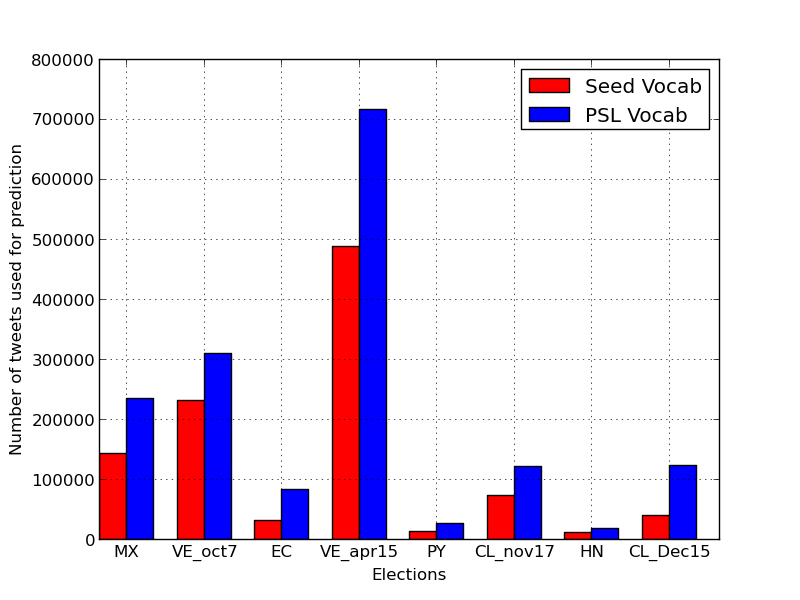
\includegraphics[width=0.7\textwidth, height=0.3\textheight]{support_files/Recall.png}
\vspace{-1em}
	\caption{Recall of seed vocabulary vs PSL vocabulary}
	\label{fig:recall}
	\vspace{-1em}
\end{figure*}
Figure \ref{fig:recall} shows the increase in the number of documents that were used by the algorithm to make a prediciton.
It is noticed when averaged across all the 8 elections we have close to a 2x increase in the number of tweets that were used by these models.
This is a substantial increase in the recall of relevant tweets for the domain.
To further illustrate the fact that the vocabulary used by such algorithms plays a vital role, we compare the performance of the models using the two different vocabularies.
The Mean Absolute Percentage Error (MAPE) was used as a metric to measure the performance of the models. 
To reduce the effect of outliers we track the popularity of only the major candidates and ignore the ones who obtained less than 10\% of the total votes.
Table \ref{table:improvement} shows the performance of each vocabulary in different elections. 
On an average it is seen that the mean absolute percentage error is reduced by 15.58\%.
